この章ではFDPSの概要を記述する。FDPSの開発目的、FDPSの基本的な考えかた、FDPSを使用して作成したコードの動作について概説する。

%%%%%%%%%%%%%%%%%%%%%%%%%%%%%%%%%%%%%%%%%%%%%%%%%%%%%%
\section{開発目的}

粒子シミュレーションは、重力$N$体シミュレーション、SPHシミュレーション、渦糸法、MPS法、分子動力学シミュレーションなど理学工学の様々な分野で使用されている。より大きい空間スケール、より高い空間分解能(または質量分解能)、より長い時間スケールの物理現象を追跡するために、高性能な粒子シミュレーションコードへの要請はますます強くなっている。

高性能な粒子シミュレーションコードを組むためには、シミュレーションコードの大規模並列化を避けることはできない。粒子シミュレーションコードの大規模並列化をする際には、ロードバランスのため動的領域分割、領域分割に合わせた粒子交換、ノード間通信の削減と最適化、キャッシュ利用効率の向上、SIMDユニット利用効率の向上、アクセラレータへの対応など、数多くの困難な処理を行う必要がある。現在、研究グループは個別にこれらの処理へ対応している。

しかし、上記の処理は粒子シミュレーション共通のものである。FDPSの開発目的は、これらの処理を高速に行うライブラリを提供し、大規模並列化への対応に追われていた研究者の負担を軽くすることである。FDPSを使うことで、研究者がよりクリエイティブな仕事に専念できるようになれば、幸いである。

%%%%%%%%%%%%%%%%%%%%%%%%%%%%%%%%%%%%%%%%%%%%%%%%%%%%%%%
\section{基本的な考えかた}

ここではFDPSの基本的な考えかたについて記述する。

%%%%%%%%%%%%%%%%%%%%%%%%%%%%%%%%%%%%%%%%%%%%%%%%%%%%
\subsection{大規模並列粒子シミュレーションの手順}
\label{subsec:pcr_of_massively_parallel_ptcl_sim}

まずFDPSにおいて、大規模並列粒子シミュレーションがどのような手順で行われることを想定しているかを記述する。粒子シミュレーションは、以下のような微分方程式を時間発展させるものである。
\begin{align}
    \frac{d\bm{u}_i}{dt} = \sum_j f(\bm{u}_i,\bm{u}_j) + \sum_s
    g(\bm{u}_i,\bm{v}_s) \label{eq:GoverningEquation}
\end{align}
ここで$\bm{u}_i$は粒子$i$の物理量ベクトルであり、この物理量には質量、位置、速度など粒子が持つあらゆる物理量が含まれる。関数$f$は粒子$j$から粒子$i$への作用を規定する。以後、作用を受ける粒子を$i$粒子、作用を与える粒子を$j$粒子と呼ぶことにする。$\bm{v}_s$は$i$粒子から十分遠方にある粒子を1つの粒子としてまとめた粒子(以後、この粒子を超粒子と呼ぶ)の物理量ベクトルである。関数$g$は超粒子から$i$粒子への作用を規定する。式(\ref{eq:GoverningEquation})の第2項は、重力やクーロン力など無限遠まで到達する長距離力の場合はゼロではない。しかし流体の圧力のような短距離力はゼロである。

大規模並列化された粒子シミュレーションコードは以下の手順で式(\ref{eq:GoverningEquation})を時間発展させる。ここではデータの入出力や初期化は省略している。
\begin{enumerate}
\item 以下の2段階の手順でどのプロセスがどの粒子の式
  (\ref{eq:GoverningEquation})を時間発展させるか決める。
  \label{item:LoadBalance}
  \begin{enumerate}
  \item プロセスの間でロードバランスを取れるように、シミュレーションで
    扱っている空間の領域を分割し、各プロセスの担当領域を決める(領域分
    割)。
  \item 各プロセスが、自分の担当する領域に存在する全粒子の物理量ベクト
    ル$\bm{u}_i$を持つように、他のプロセスと物理量ベクトル$\bm{u}_i$を
    交換する(粒子交換)。
  \end{enumerate}

\item 各プロセスは、自分の担当する全粒子の式
  (\ref{eq:GoverningEquation})の右辺を計算するのに必要な$j$粒子の物理
  量ベクトル$\bm{u}_j$と超粒子の物理量ベクトル$\bm{v}_s$を他のプロセス
  と通信することで集めて、$j$粒子のリストと超粒子のリスト(まとめて相互
  作用リストと呼ぶ)を作る(相互作用リストの作成)。
  \label{item:MakeInteractionList}

\item 各プロセスは自分の担当する全粒子に対して、式
  (\ref{eq:GoverningEquation})の右辺を計算し、$d\bm{u}_i/dt$を求める
  (相互作用の計算)。\label{item:CalcInteraction}

\item 各プロセスは、自分の担当する全粒子の物理量ベクトル$\bm{u}_i$とそ
  の時間導関数$d\bm{u}_i/dt$を使って、全粒子の時間積分を実行し、次の時
  刻の物理量ベクトル$\bm{u}_i$を求める(時間積分)。
  \label{item:IntegrateTime}

\item 手順\ref{item:LoadBalance}に戻る。        
\end{enumerate}

%%    ただし、あらゆる相互作用のタイプに対応するには以下5種類の$j$粒子
%%    と超粒子の集め方が必要。\label{item:MakeInteractionList}    
%%    \begin{itemize}
%%        \item 長距離力モード:$i$粒子に対して、近い粒子は$j$粒子として、
%%        遠方の複数の粒子はまとめて超粒子として集めるモード(使用例:開
%%        放条件下の重力やクーロン力)
%%        \item 長距離力モードカットオフ付き:長距離力モードとほぼ同じだ
%%        が、ある距離より遠い粒子は集めないモード(使用例:周期境界条件
%%        下の重力やクーロン力)
%%        \item 短距離力収集モード:$i$粒子自身の持つサーチ半径の内側に
%%        ある粒子のみ$j$粒子として集めるモード(使用例:SPH法における密
%%        度の計算)
%%        \item 短距離力散乱モード:$i$粒子をサーチ半径の内側に含む粒子
%%        を$j$粒子として集めるモード(使用例:Lennard-Jones力)
%%        \item 短距離力対称モード:短距離力収集モードで集める粒子と短距
%%        離力散乱モードで集める粒子の和集合を$j$粒子として集めるモード
%%        (使用例:SPH法における圧力勾配の計算)    
%%    \end{itemize}

%%%%%%%%%%%%%%%%%%%%%%%%%%%%%%%%%%%%%%%%%%%%%%%%%%%%
\subsection{ユーザーとFDPSの役割分担}

FDPSは、プロセス間の通信が発生する処理はFDPSが担当し、プロセス間の通信の発生しない処理はユーザーが担当するという役割分担を基本としている。従って、前節に挙げた、領域分割・粒子交換(項目\ref{item:LoadBalance})・相互作用リストの作成(項目\ref{item:MakeInteractionList})をFDPSが、相互作用の計算(項目\ref{item:CalcInteraction})・時間積分(項目\ref{item:IntegrateTime})をユーザーが担当することになる。ユーザーはFDPSのAPIを呼び出すだけで、大規模並列化に関わる煩雑な処理を避けつつ、高性能な任意の相互作用の粒子シミュレーションコードを手に入れることができる。

%%%%%%%%%%%%%%%%%%%%%%%%%%%%%%%%%%%%%%%%%%%%%%%%%%%%
\subsection{ユーザーのやること}
\label{subsec:things_to_do_by_users}

ユーザーがFDPSを使って粒子シミュレーションコードを作成するときにやるこ
とは以下の項目である。
\begin{itemize}

%%\item 座標系の選択(節\ref{sec:compile_coordinate})。2次元または3次元
%%  直角座標系の選択が可能。

%%\item 境界条件の選択(節\ref{sec:datatype_enum_boundarycondition})。開
%%  放境界条件、x, y, z軸方向どれかまたはすべての周期境界条件の選択が可
%%  能。
    
\item 粒子の定義(第\ref{chap:user_defined}章)。粒子の持つ物理量(式
  (\ref{eq:GoverningEquation})で言えば$\bm{u}_i$)の指定。例えば質量、
  位置、速度、加速度、元素組成、粒子サイズ、など。

\item 相互作用の定義(第\ref{chap:user_defined}章)。粒子間の相互作用(式
  (\ref{eq:GoverningEquation})で言えばで関数$f$, $g$)を指定。例えば、
  重力、クーロン力、圧力、など。

\item FDPSのAPIの呼出(第\ref{chap:API_spec_list}章)

\end{itemize}

%%%%%%%%%%%%%%%%%%%%%%%%%%%%%%%%%%%%%%%%%%%%%%%%%%%%
\subsection{補足}

式(\ref{eq:GoverningEquation})の右辺は2粒子間相互作用の重ね合わせである。従って、FDPSのAPIを呼ぶだけでは、3つ以上の粒子の間の相互作用の計算を行うことはできない。しかし、FDPSはネイバーリストを返すAPIを用意している。ネイバーリストを用いれば、ユーザーはプロセス間の通信の処理をすることなく、このような相互作用の計算をできる。

第\ref{subsec:pcr_of_massively_parallel_ptcl_sim}節で示した手順は、全粒子が同じ時間刻みを持っている。そのため、FDPSのAPIを呼び出すだけでは、独立時間刻みで時間積分を効率的に行うことができない。しかし、上と同じくネイバーリストを返すAPIがあるため、Particle Particle Particle Tree法を用いて独立時間刻みを実装することは可能であろう。

%%マルチプロセス, マルチスレッド, SIMD演算を用いて, 並列に処理される.
%%FDPSはC++言語にて記述される.

%%%%%%%%%%%%%%%%%%%%%%%%%%%%%%%%%%%%%%%%%%%%%%%%%%%%%
\section{コードの動作}
\label{sec:overview_action}
ここではFDPSを使用して作成したコードの動作の概略を記述する。まずはじめにC++で記述されたFDPS本体の動作の概略を説明し、その後、Fortran/C言語 インターフェースの動作を解説する。
%%%%%
\subsection{FDPS 本体}
FDPS本体のコードには4つのモジュール\footnote{1つの大きな機能を提供するためのデータと手続きの集まりという意味。FDPSではモジュールをC++のクラス機能によって実現している。}がある。3つはFDPSのモジュールで、1つはユーザー定義のモジュールである。まとめると以下のようになる。
\begin{itemize}
\item 領域クラス:全プロセスが担当する領域の情報と、領域分割を行うAPI
  を持つ
\item 粒子群クラス:全粒子の情報と、プロセスの間での粒子交換を行うAPI
  を持つ
\item 相互作用ツリークラス:粒子分布から作られたツリー構造と、相互作用
  リストを作成するAPIを持つ
\item ユーザー定義クラス:ある1粒子を定義するクラス、粒子間の相互作用
  を定義する関数オブジェクトを持つ
\end{itemize}

これら4つのモジュールの間で情報がやり取りされる。これは図\ref{fig:brief_interface}で概観できる。図\ref{fig:brief_interface}に示された情報のやりとりは、第\ref{subsec:pcr_of_massively_parallel_ptcl_sim}節に記述された手順\ref{item:LoadBalance}から\ref{item:CalcInteraction}と、これらの手順以前に行われる手順(手順0とする)に対応する。
以下はこれらの手順の詳細な記述である。
\begin{enumerate}
\item[0.] ユーザー定義クラスのうち1粒子を定義するクラスが粒子群クラスへ、粒子間の相互作用を定義する関数オブジェクトが相互作用ツリークラスへ渡される。これはクラスの継承ではなく、粒子を定義するクラスは粒子群クラスのテンプレート引数として、粒子間の相互作用を定義する関数オブジェクトは相互作用ツリークラスのAPIの引数として渡される
\item[\ref{item:LoadBalance}.] 以下の2段階でロードバランスを取る
  \begin{enumerate}
  \item 領域クラスが持つ領域分割のAPIが呼ばれる。このとき粒子情報が粒子群クラスから領域クラスへ渡される (赤字と赤矢印)
  \item 粒子群クラスが持つ粒子交換のAPIが呼ばれる。このとき領域情報が領域クラスから粒子群クラスへ渡される (青字と青矢印)
  \end{enumerate}
\item[\ref{item:MakeInteractionList}.] 相互作用ツリークラスが持つ相互作用リストを作成するAPIが呼ばれる。このとき領域情報が領域クラスから相互作用ツリークラスへ、粒子情報が粒子群クラスから相互作用ツリークラスへ渡される (緑字と緑矢印)
\item[\ref{item:CalcInteraction}.] 相互作用ツリーククラスが持つ相互作用を定義した関数オブジェクトを呼び出すAPIが呼ばれる。相互作用計算が実行され、相互作用計算の結果が相互作用ツリークラスから粒子群クラスへ渡される (灰色の字と灰色矢印)
\end{enumerate}

\begin{figure}[h]
\centering
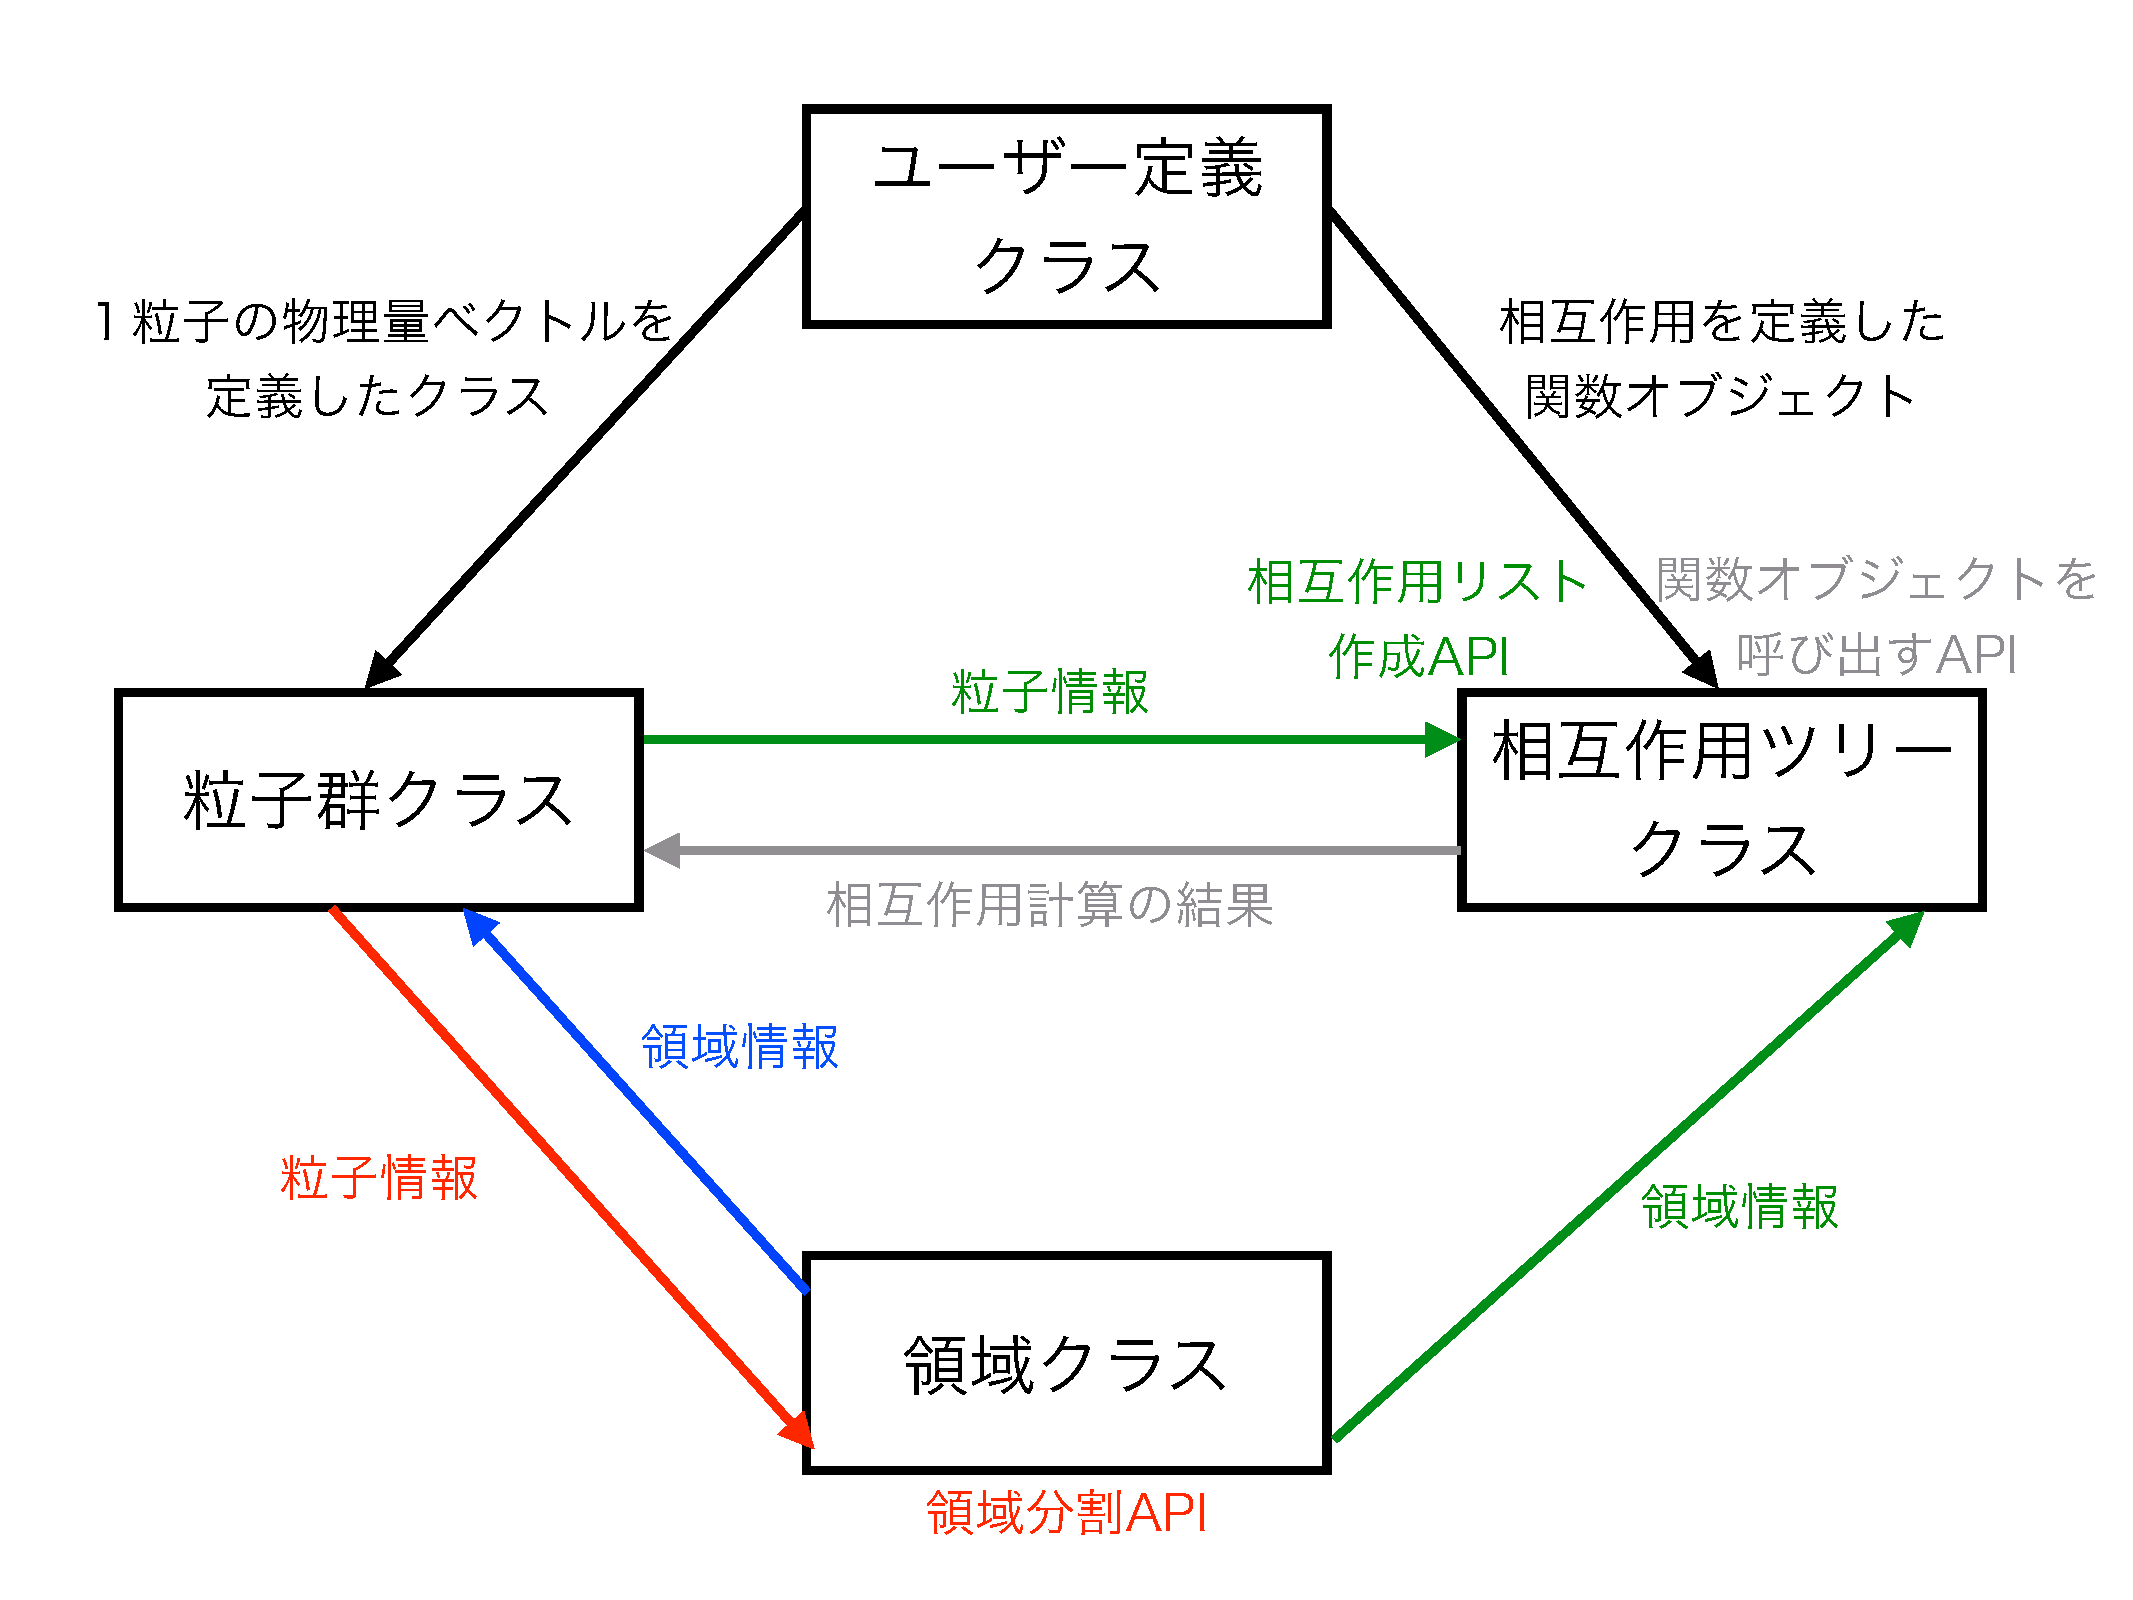
\includegraphics[width=0.75\linewidth]{./fig/illustration/illustration.pdf}
\caption{モジュールインターフェースと情報の流れの模式図。}
\label{fig:brief_interface}
\end{figure}

%%%%%
\subsection{Fortran/C言語 インターフェース}
次章以降で詳しく述べるが、前節で述べたAPIはFortranインターフェース及びC言語インターフェースにも用意されている。したがって、Fortran或いはC言語においても、第\ref{subsec:pcr_of_massively_parallel_ptcl_sim}節に記述された手順は、対応するAPIの適切な呼び出しにより実現できる。


